\newpage
\subsection{Оперативное планирование продаж}
\label{bp:salesplan}




Генеральный директор даёт ограничение по плану продаж на каждый месяц.
В системе 1С:УПП создается оперативный продаж на каждый месяц (см. \ref{pic:d1}).
План продаж определяет генеральный директор.
В форме представлены плановые показатели по продажам, фактическая величина отгрузки, просроченная задолженность по покупателю.


% При появлении от клиентов заявок от покупателей менеджеры регистрируют в системе СБИС документ ''Заявка покупателя'' (рис. \ref{pic:dd9}). Менеджеры формируют при необходимости счет на оплату из формы документа \ref{pic:dd8} или создают документ «Счет». 

% В системе СБИС менеджеры регистрируют все заявки покупателя.

% %Выделено несколько крупных покупателей, по которым до 25 числа каждого месяца требуется создавать заявки покупателей в 1С: УПП. Таких клиентов только 50\%. 
% Составление списка заявок покупателей в системе СБИС 
% % на начало месяца 
%  можно условно назвать 
% % является 
% оперативным планирование продаж.
% %
% %






%Ежемесячно менеджеры отдела сбыта и логистики совместно с коммерческим директором разрабатывают оперативный план. 

% Разрез планирования: виды выпускаемой продукции, декада месяца.
% Показатель планирования: метры квадратные по готовой продукции.
 
%Позаказный учет отсутствует.
 
%Для каждой позиции указывается заказчик, размеры изделия, марка, оснастка, композиция сырья, план в производство и факт производства и отгрузки.

%План создается по каждому менеджеру. Оперативный план продаж является документом, по которому формируются все дальнейшие планы: план производства, план работы гофроагрегата, план работы перерабатывающих линий, план потребности в материалах, план отгрузки.
%Форма плана приведена на рис. \ref{pic:salesplan}.
%
\begin{figure}
\begin{center}
 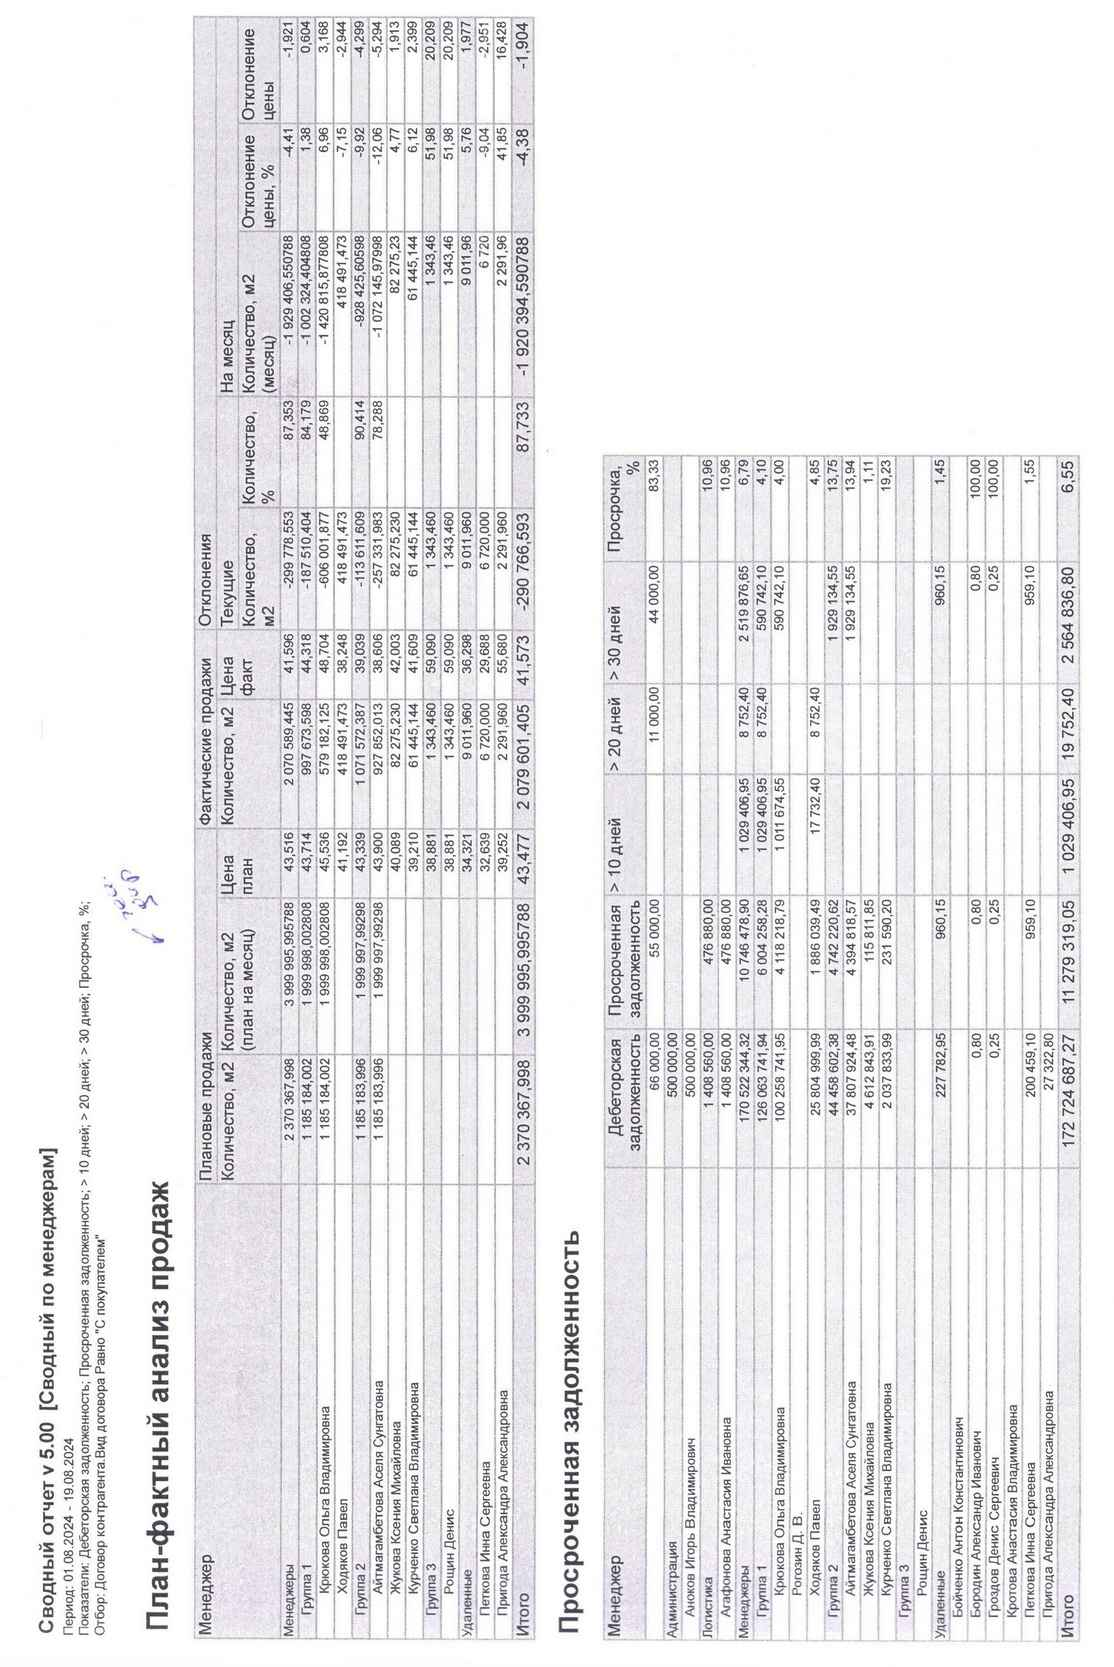
\includegraphics[height=0.94\textheight, width=0.9\textwidth,  keepaspectratio]{Pics/d01.jpg}
\end{center}
 \caption{План продаж на месяц по каждому менеджеру}
 \label{pic:d1}
\end{figure}
\clearpage


% \begin{figure}
% \begin{center}
%  \includegraphics[height=0.94\textheight, width=0.9\textwidth,  keepaspectratio]{Pics/pic.jpg}
% \end{center}
%  \caption{Цепочка заказов для планирования}
%  \label{pic:pic_d14}
% \end{figure}
% \clearpage

%
%



%Оперативное планирование определяется на основе формы \ref{pic:monthplan}, куда менеджер фиксирует все поступающие заявки.
%Производство каждый день  сообщает менеджерам коммерческого отдела  результаты работы производства. 
%При этом плановик  звонит менеджеру коммерческого отдела и говорит какие заказы приняты в производство на текущую дату.
%%Специалисты отдела планирования сообщают план выполнения на 2 дня. 
%Планировщик сообщает дату, на которую поставлен заказ. Так менеджеры узнают, когда их заявка покупателя поставлена в работу. 
%Дата (период) производства в форме плана  (см рис. \ref{pic:monthplan}) уже согласована.
%В программе 1С менеджер создает надокумент ''Счет''  и печатает форму заказа на отгрузку, в котором указывает дату отгрузки, адрес доставки, номенклатуру продукции, цены, объём. 


%\begin{figure}
%\begin{center}
%  \includegraphics[height=0.94\textheight, keepaspectratio]{Pics/prodline_loading.jpg}
%\end{center}
%  \caption{Отчет по загруженности линий}
%  \label{pic:prodline_loading}
%\end{figure}

\clearpage
\ifx \notincludehead\undefined
\normalsize
\end{document}
\fi